% !TeX TS-program = xelatex
\documentclass[aspectratio=169, 12pt, xcolor=table]{beamer}
\usefonttheme{professionalfonts}
\usefonttheme{serif}
\usepackage[T1]{fontenc}
\usepackage{fontspec-xetex}

\usepackage{booktabs}
\usepackage{listings}
\usepackage{subcaption}

\setmainfont{Lato}

%\PassOptionsToPackage[more=table]{xcolor}

% Local configuration
\renewcommand{\figurename}{}
\DeclareCaptionFormat{custom}
{%
	\tiny #3
}
\captionsetup{format=custom}

% Title stuff
\title{Statistical Techniques}
\subtitle{Multilinear Regression}
\date{Week 06}
\author{Vassilis Markos, Mediterranean College}

\usetheme{streamline}
%\usepackage{/theme/beamerthemestreamline}

% Local Commands
\newcommand{\ohref}[1]{\href{#1}{\texttt{#1}}}
\def\sms#1{\smsgo#1\relax}
\def\smsgo#1.#2\relax{#1.{\scriptsize #2}}

% Code listings

\definecolor{codegreen}{rgb}{0,0.6,0}
\definecolor{codegray}{rgb}{0.5,0.5,0.5}
\definecolor{codepurple}{rgb}{0.58,0,0.82}
\definecolor{backcolour}{rgb}{0.95,0.95,0.92}

\lstdefinestyle{mystyle}{
	backgroundcolor=\color{backcolour},   
	commentstyle=\color{codegreen},
	keywordstyle=\color{magenta},
	numberstyle=\tiny\color{codegray},
	stringstyle=\color{codepurple},
	basicstyle=\ttfamily\footnotesize,
	breakatwhitespace=false,         
	breaklines=true,                 
	captionpos=b,                    
	keepspaces=true,                 
	numbers=left,                    
	numbersep=5pt,                  
	showspaces=false,                
	showstringspaces=false,
	showtabs=false,                  
	tabsize=2
}

\lstset{style=mystyle}

\begin{document}

	\begin{frame}
		\titlepage
	\end{frame}

	\begin{frame}{Contents}
		\tableofcontents
	\end{frame}

	\section{Last Time's Recap}\label{sec:last-time-recap}
	
	\sectionframe
	
	
	\begin{frame}{mpg vs weight}
		\begin{center}
			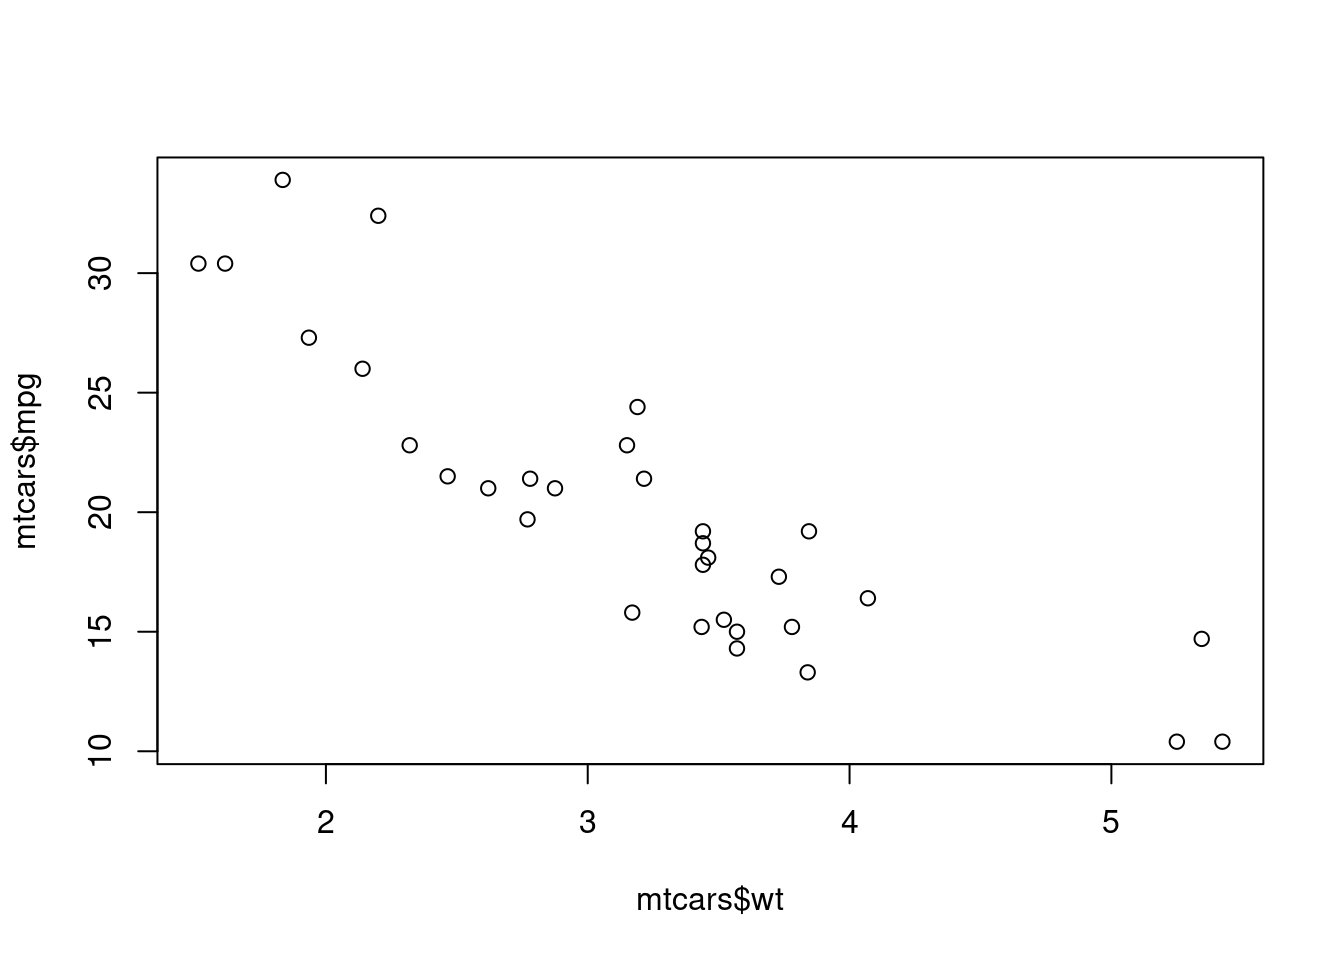
\includegraphics[width=0.65\textwidth]{img/mpgwt.png}
		\end{center}
	\end{frame}

	\begin{frame}[fragile]{A Linear Model}
		
		\lstinputlisting[language=R, linerange={20-21}]{src/lg.Rmd}
		
		\begin{tiny}
\begin{verbatim}
Call:
lm(formula = mpg ~ wt, data = mtcars)

Residuals:
Min      1Q  Median      3Q     Max 
-4.5432 -2.3647 -0.1252  1.4096  6.8727 

Coefficients:
Estimate Std. Error t value Pr(>|t|)    
(Intercept)  37.2851     1.8776  19.858  < 2e-16 ***
wt           -5.3445     0.5591  -9.559 1.29e-10 ***
---
Signif. codes:  0 ‘***’ 0.001 ‘**’ 0.01 ‘*’ 0.05 ‘.’ 0.1 ‘ ’ 1

Residual standard error: 3.046 on 30 degrees of freedom
Multiple R-squared:  0.7528,    Adjusted R-squared:  0.7446 
F-statistic: 91.38 on 1 and 30 DF,  p-value: 1.294e-10
\end{verbatim}
		\end{tiny}
		
	\end{frame}


	\begin{frame}{How Does Our Model Look Like?}
		\begin{itemize}
			\item To plot our model over the scattered data points, we have to plot both one on top of the other.
			\item Remember to plot your variables the same way they appear in your model, i.e., $y$ against $x$, otherwise, you might get a non-sensical plot!
		\end{itemize}
		
		\lstinputlisting[language=R, linerange={25-26}]{src/lg.Rmd}
	\end{frame}


	\begin{frame}{Our Model!}
		\begin{center}
			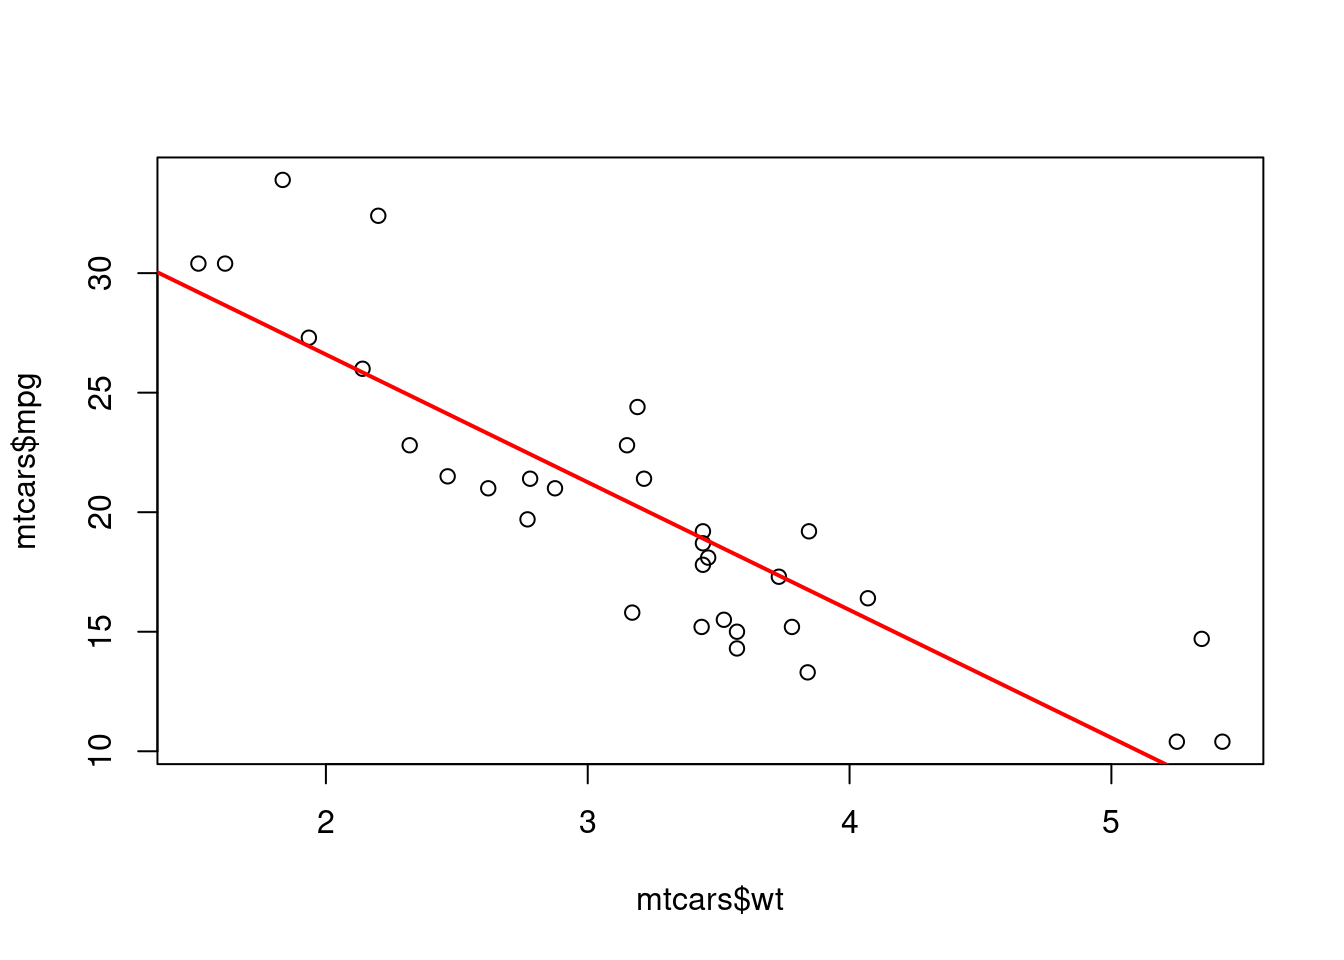
\includegraphics[width=0.75\textwidth]{img/model.png}
		\end{center}
	\end{frame}

	\begin{frame}{Residuals vs Fitted}
		\begin{center}
			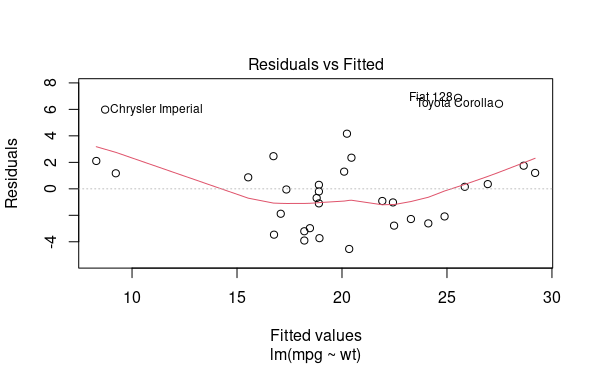
\includegraphics[width=0.75\textwidth]{img/rsdfit.png}
		\end{center}
	\end{frame}


	\begin{frame}{Normal Q-Q}
		\begin{center}
			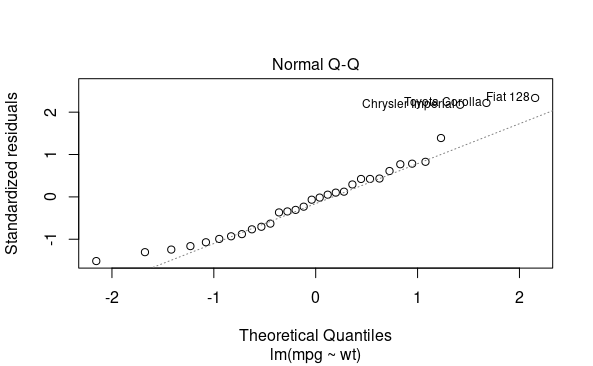
\includegraphics[width=0.75\textwidth]{img/qq.png}
		\end{center}
	\end{frame}


	\begin{frame}{Scale-Location}
		\begin{center}
			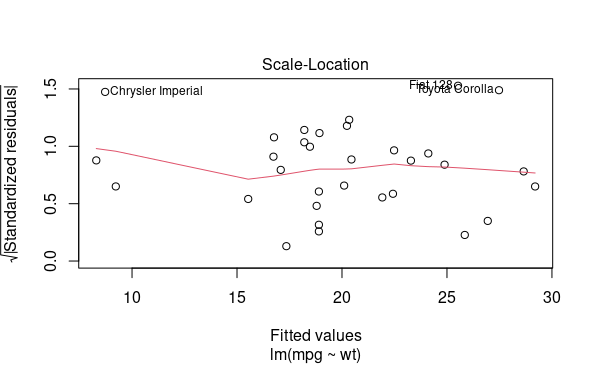
\includegraphics[width=0.75\textwidth]{img/sl.png}
		\end{center}
	\end{frame}


	\begin{frame}{Residuals vs Leverage}
		\begin{center}
			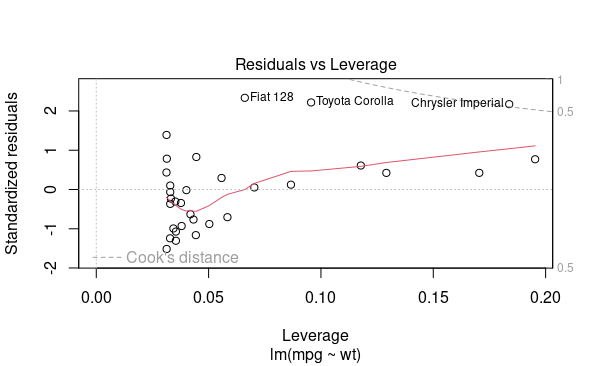
\includegraphics[width=0.75\textwidth]{img/rl.png}
		\end{center}
	\end{frame}

	\begin{frame}{Don't Rely Just on Regression!}
		\begin{center}
			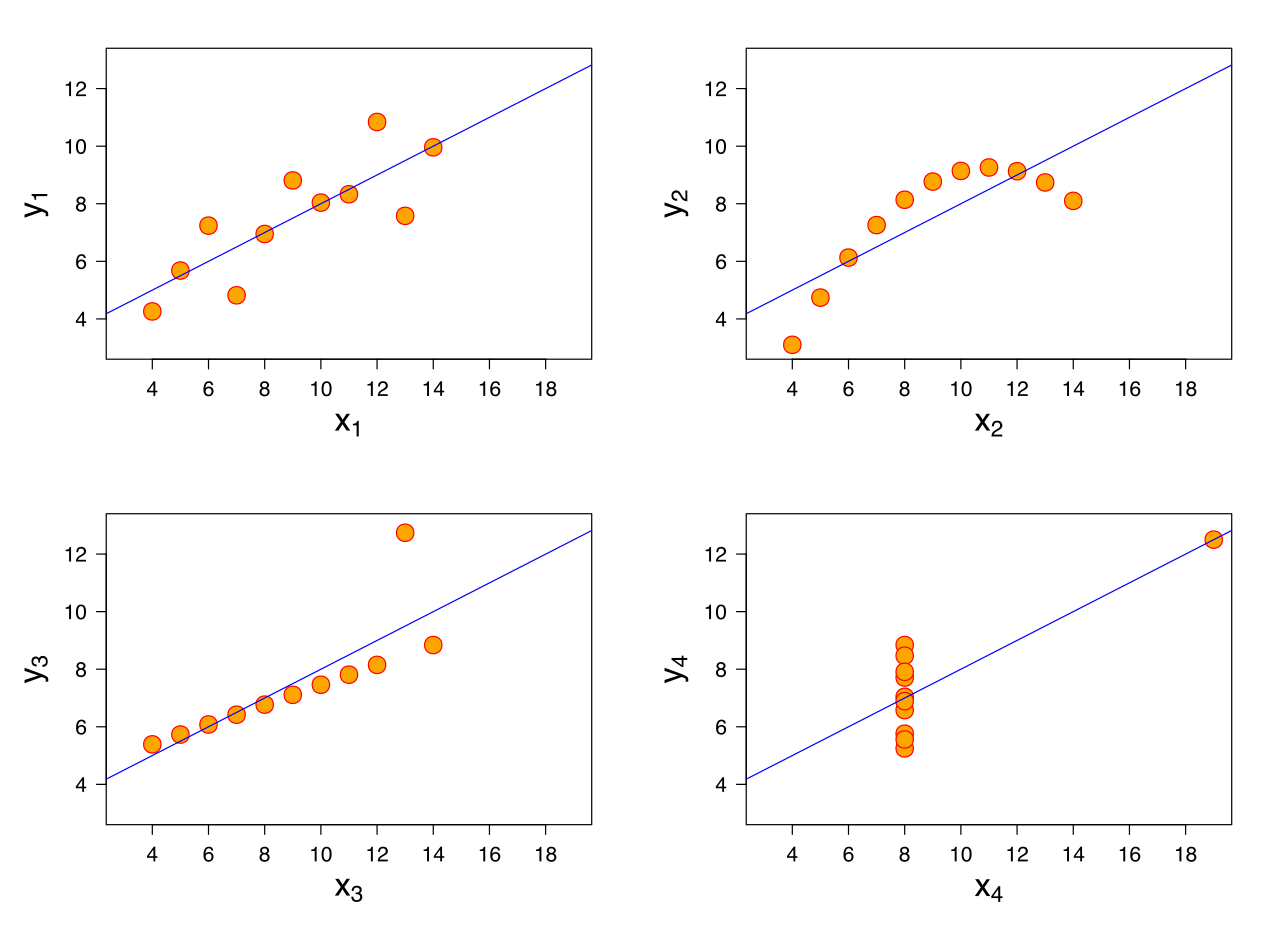
\includegraphics[width=0.5\textwidth]{img/anscombe.png}
		\end{center}
		{\tiny Source: \url{https://en.wikipedia.org/wiki/Linear_regression\#Least-squares_estimation_and_related_techniques}}
	\end{frame}

	\section{Multilinear Regression}
	
	\sectionframe
	
	\begin{frame}{Taking a Fresh Look}
		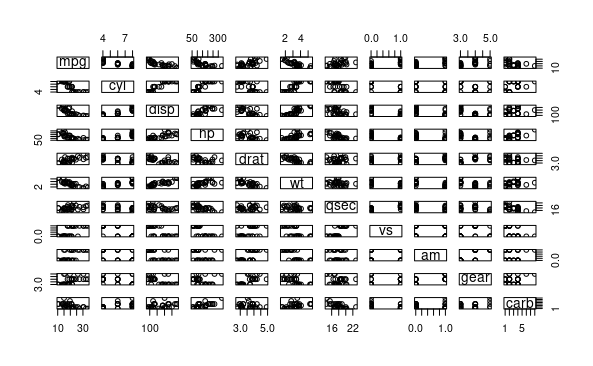
\includegraphics[width=0.75\textwidth]{img/pairs.png}
	\end{frame}

	\begin{frame}{mpg vs HP}
		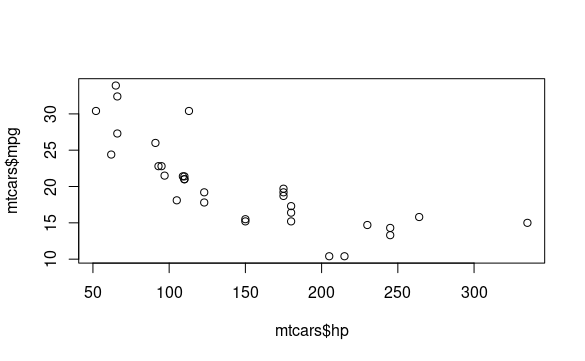
\includegraphics[width=0.75\textwidth]{img/mpghp.png}
	\end{frame}

	\begin{frame}{mpg vs Rear axle ratio}
		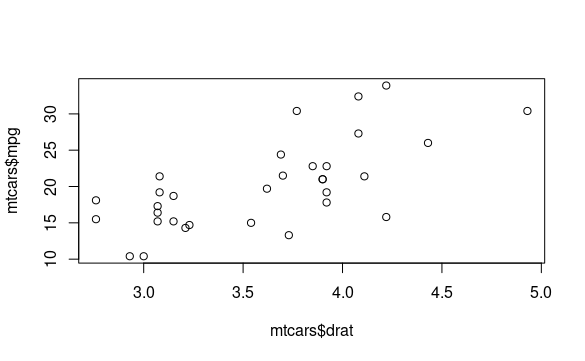
\includegraphics[width=0.75\textwidth]{img/mpgdrat.png}
	\end{frame}
	
	\begin{frame}{Linearities}
		\begin{itemize}
			\item There is a chance that both \texttt{hp} and \texttt{drat} are linearly related to \texttt{mpg}.
			\item One way to investigate this would be to create two more linear models, as we did last time for \texttt{mpg} and \texttt{wt}.
			\item Can you see any issues with that?\pause
			\item Evidently, we are not taking into account potential compound effects.
		\end{itemize}
	\end{frame}

	\begin{frame}{Multiple Linear Regression}
		\begin{itemize}
			\item As with (simple) linear regression, in MLR we make some similar assumptions.
			\item To begin with, we assume that residuals are normally distributed. Again, we can verify this only after we have computed the model, e.g., through Q-Q plots.
			\item We further assume that there actually are linear relationships between the predicted and the predicting variables (visually demonstrating this, usually).
		\end{itemize}
	\end{frame}
	
	\begin{frame}{Multiple Linear Regression}
		\begin{itemize}
			\item We also assume \textbf{multicollinearity}, i.e., that the predicting variables are not that highly correlated with one another. We typically check this using Correlation Matrices and looking for values in $(-0.8,0.8)$.
			\item We need to further assume \textbf{homoscedasticity}, i.e., that the variance (-scedasticity) of the various independent variables is uniformly distributed across them (homo-).
			\begin{itemize}
				\item How can we test this visually?\pause
				\item Plots like the scale-location plot come in handy here.
			\end{itemize}
		\end{itemize}
	\end{frame}

	\begin{frame}{The Maths Behind All This Stuff}
		Let $\vec{x}=[x_1,x_2,\ldots,x_n]$ be some independent variables and $y$ be dependent variable we are trying to predict. Then, we are looking for $\vec{\beta}=[\beta_0,\beta_1,\ldots,\beta_n]$ such that:
		\[y=\beta_0+\beta_1x_1+\cdots+\beta_nx_n=\beta_0+\sum_{i=1}^n\beta_ix_i=\beta_0+\vec{\beta}\cdot\vec{x}.\]
		Since this $\beta_0$ is looking so lonely in the above formula, we redefine $\vec{x}=[1,x_1,x_2,\ldots,x_n]$ (prepending a $1$), so, we have:
		\[y=\vec{\beta}\cdot\vec{x}.\]
	\end{frame}

	\begin{frame}{The Maths Behind All This Stuff}
		Now, let $y_i$ denote the $i$-th observation and $\vec{x}_i$ be the corresponding observations on the independent variables. Then, as in the (simple) linear case, we have:
		\[y_i=\vec{\beta}\cdot\vec{x}_i+\varepsilon_i,\quad i=1,\ldots,m.\]
		Using all the extended observation vectors $\vec{x}_i$, we can build a matrix:
		\[X=[\vec{x_1};\cdots;\vec{x_n}]=\left[\begin{array}{cccc}
			1 & 1 & \cdots & 1 \\
			x_1^1 & x_2^1 & \cdots & x_n^1\\
			\vdots & \vdots & \ddots & \vdots \\
			x_1^m & x_2^m & \cdots & x_n^m
		\end{array}\right].\]
	\end{frame}

	\begin{frame}{The Maths Behind All This Stuff}
		Denoting the corresponding dependent variable and coefficient columns as:
		\[Y=\left[\begin{array}{c}
			y_1 \\ y_2 \\ \vdots \\ y_m
		\end{array}\right],\quad \vec{\beta}=\left[\begin{array}{c}
			\beta_0 \\ \beta_1 \\ \vdots \\ \beta_n
		\end{array}\right],\]
		we can find with common multivariate calculus optimisation that:
		\[\hat{\beta}=(X^TX)^{-1}X^TY.\]
	\end{frame}

	\section{Application on \texttt{mtcars}}
	
	\sectionframe
	
	\begin{frame}[fragile]{All This, Just Using R}
		\lstinputlisting[language=R, linerange={208-209}]{src/notes.Rmd}
		
\begin{tiny}
		\begin{verbatim}
Call:
lm(formula = mpg ~ wt + hp + drat, data = mtcars)

Residuals:
Min      1Q  Median      3Q     Max 
-3.3598 -1.8374 -0.5099  0.9681  5.7078 

Coefficients:
Estimate Std. Error t value Pr(>|t|)    
(Intercept) 29.394934   6.156303   4.775 5.13e-05 ***
wt          -3.227954   0.796398  -4.053 0.000364 ***
hp          -0.032230   0.008925  -3.611 0.001178 ** 
drat         1.615049   1.226983   1.316 0.198755    
---
Signif. codes:  0 ‘***’ 0.001 ‘**’ 0.01 ‘*’ 0.05 ‘.’ 0.1 ‘ ’ 1

Residual standard error: 2.561 on 28 degrees of freedom
Multiple R-squared:  0.8369,    Adjusted R-squared:  0.8194 
F-statistic: 47.88 on 3 and 28 DF,  p-value: 3.768e-11
\end{verbatim}
\end{tiny}
	\end{frame}

	\begin{frame}{Fun Time!}
		\begin{itemize}
			\item We have seen all the corresponding assessment measures last time, so, now it's your turn to assess this model!
			\item Judging by its summary, what can you tell about the linear dependence between the \texttt{mpg} and the three variables chosen? Was out intuition correct?
			\item Use plots and all other tools we explored last time to justify your decision.
			\item Amend / Change the model, if needed, maybe dropping some variables.
		\end{itemize}
	\end{frame}
	
\end{document}